  %%%%%%%%%%%%%%%%%%%%%%%%%%%%%%%%%%%%%%% -*- coding: utf-8; mode: latex -*- %%
  %
%%%%%                         CHAPTER
 %%%
  %

% $Id: 1020-lorem-ipsum.tex,v 1.2 2009/06/19 15:51:46 david Exp $
% $Log: 1020-lorem-ipsum.tex,v $
% Revision 1.2  2009/06/19 15:51:46  david
% *** empty log message ***
%
% Revision 1.1  2007/11/23 09:52:39  david
% *** empty log message ***
%
%

  %%%%%%%%%%%%%%%%%%%%%%%%%%%%%%%%%%%%%%%%%%%%%%%%%%%%%%%%%%%%%%%%%%%%%%%%%%%%%
  %
%%%%%                           HEAD MATTER
 %%%
  %

\chapter{Read-Only Nested Snapshots}
%\addcontentsline{lof}{chapter}{\thechapter\quad Lorem Ipsum}
%\addcontentsline{lot}{chapter}{\thechapter\quad Lorem Ipsum}
\label{ch:RONSSolution}

This section presents solution to Netsed Snapshots problem disussed in \ref{ch:RONSProblem}
  %%%%%%%%%%%%%%%%%%%%%%%%%%%%%%%%%%%%%%%%%%%%%%%%%%%%%%%%%%%%%%%%%%%%%%%%%%%%%
  %
%%%%%                        FIRST SECTION
 %%%
  %
\section{Snapshottable Directories}

 These are directories that are configured
by the system administrator to allow snapshots. A snapshot can be created only at these snapshot roots
instead of at arbitrary directories.
Directories that are marked snapshottable cannot be deleted until all the snapshots under that directory
are deleted. Similarly, another directory cannot be renamed to an existing a snapshottable directory
that has snapshots (since rename involves deletion of the rename target). The above restrictions
simplify the design by not having to deal with how to mange a snapshot when the snapshottable
directory is deleted and no longer exists or worst still a new directory with the same name is created in
its place.

\section{Modifications to the Schema}
\label{RONSS:schema}

Following columns need to be added to the Inodes table described in the schema \ref{fig:HDFS_table_schema} of HOP File System.
\begin{enumerate}
\item isDeleted \\\\
\begin{tabular}{|c|p{15cm}|}
\hline
Value&Summary\\
\hline
0&Indicates that this Inode is not deleted.\\
\hline
1&Indicates that this Inode deleted after snapshot was taken[on its ancestors].\\ 
\hline
\end{tabular} \\
\item isSnapshottableDirectory\\\\
\begin{tabular}{|c|p{15cm}|}
\hline
Value&Summary\\
\hline
0&Indicates that snapshots can't be taken on this directory.\\
\hline
1&Indicates that snapshots can be taken on this directory.\\ 
\hline
\end{tabular} \\
\end{enumerate}
Following tables need to be added to the schema \ref{fig:HDFS_table_schema}.
\begin{enumerate}
\item \textbf{SNAPS}\\\\
\begin{tabular}{|c|c|c|c|}
\hline
Inode\_ Id&
User&
SnapShot\_ Id&
Time\\
\hline
\end{tabular}\\\\
Stores the Indode Id and corresponding snapshots taken on that directory. Time can be a physical clock or logical clock(Global) whose value always increase.

\item \textbf{C-List}\\\\
\begin{tabular}{|c|c|c|}
\hline
Inode\_ Id&
Time&
Created\_ Inode\_ Id\\
\hline
\end{tabular}\\\\
Stores the id's of children(files or directories) of directory on which snapshot was taken.



\item \textbf{D-List}\\\\
\begin{tabular}{|c|c|c|}
\hline
Inode\_ Id&
Time&
Deleted\_ Inode\_ Id\\
\hline
\end{tabular}\\\\
Stores the  files or directories  deleted in a directory on which snapshot was taken. But the rows are not deleted from Inode table, it is an indication to say that these rows were deleted after taking snapshots.

\item \textbf{M-List}\\\\
\begin{tabular}{|c|c|c|c|}
\hline
Inode\_ Id&
Time&
Modified\_ Inode\_ Id&
Original Row\\
\hline
\end{tabular}\\\\
After taking a Snapshot if the columns of a particular row are modified then before modifying the row , we copy the original row and store it in this table. When we want to get back to the snapshot, just replace the existing inode row with this original row.

\item \textbf{MV-List}\\\\
\begin{tabular}{|c|c|c|c|}
\hline
Inode\_ Id&
Time&
Moved\_ Inode\_ Id&
Original Row\\
\hline
\end{tabular}\\\\
When an inode[either file or directory] is moved, its parentId changes to moved-into directory. In order to get the moved directory when ls command issued at the snapshot after which this inode was moved, we put that row here. 

\item \textbf{MV-IN-List}\\\\
\begin{tabular}{|c|c|c|c|}
\hline
Inode\_ Id&
Time&
Moved\_ In\_ Inode\_ Id\\
\hline
\end{tabular}\\\\
When a directory or file is moved into this directory(with inode\_ id) from other directory.

\item \textbf{Block-Info-C-List}\\\\
\begin{tabular}{|c|c|c|}
\hline
Inode\_ Id&
Block\_ Id&
Time\\
\hline
\end{tabular}\\\\
Stores the blocks that are created in a file after the snapshot was taken on the directory in which this file exist.

\item \textbf{Block-Info-M-List}\\\\
\begin{tabular}{|c|c|c|c|}
\hline
Inode\_ Id&
Block\_ Id&
Time&
Original\_ Row\\
\hline
\end{tabular}\\\\
Stores the blocks that are modified in a file after the snapshot was taken on the directory in which this file exist.This is typically for last blocks which are not complete at the time of snapshot.

\end{enumerate}

\section{Rules for Operations}
\begin{enumerate}

\item  When we create a new file or directory put an entry in c-list.

\item When an inode is modified [rename, touch] it is just put in the M-List. It is not put in the D-List.

\item When you delete a file , put it in the dlist. And set isInodeDeleted to true.

\item Deleting a directory
When an directory is deleted, first we will check  whether it is in a snapshot[explained later], if yes then we will set isDeleted=1 and also for all of its childrens[recursive]. We only put the directory in D-List of its parent and we do not put children in D-List.

\item When an inode is moved to some other directory we put it in  MV-List of parent directory. We place it in MV-IN-list of destination  directory.[the parent\_ id is set to the destination directory]

\end{enumerate}

\section{Listing children under a directory in a given Snapshot}

\section{Listing current children under a directory }


\section{Logging, Removing logs and Deleting inodes which are not referred by any snapshot}

Here two approaches two solve the issues are presented.
\subsection{Approach 1:}
\textbf{Columns to be added to Inodes Table}\\
1. Moved\_ In/Created Time: When an Inode is created we put that time in that column. When we move an Inode from one directory to another we note that time in that.\\\\
\textbf{MovedPaths}\\
\begin{table}[h!]
\begin{tabular}{|c|c|c|}
\hline
Inode\_ Id&
Path&
Time\\
\hline
\end{tabular}\\
\caption{MovedPaths table}
\label{movedPaths}
\end{table}


\subsubsection{When to Log}
 When we add/ deleted/modify directories or files in a directory then we log changes under that directory. We log only when this directory is in any snapshot[which is taken on this directory or one-of its ancestors]. So before performing any operation in this directory we check whether this directory is in any snapshot or not. We take help of the table MovedPaths \ref{movedPaths}.Ex: we have /A/B/C/ as path, where A,B, and C are directories.Suppose we want to add a file in C. Now we need to check whether C is in any snapshot. On a first sight, we can think that checking whether any snapshots taken on A,B,C before C was created , but B or A may be moved from different place, for example B may be moved from /A/D/ path and there may be some snapshots taken on directory D even though no snapshots may be not taken on A and B. To handle that situation, whenever we move a file or directory, first we check whether it is in a snapshot, if yes then insert a row in the MovedPaths table containing original path before being moved. \\
 Assume following path exist /U/V/W/X [U,V,W,X are directories, we are performing add/delete/modify on inodes(files or directories) in it]. Say we are performing operation on inode P whose path is /U/V/W/X/P.First, we need to find whether P is in any snapshot. We find that with below steps.If P is in any snapshot then we log the operation in corresponding table which are described above \ref{RONSS:schema}. 
 \begin{enumerate}
 \item  Check if any snapshots on U,V,W,X before present time.
\item  If we not find any in step1 then check in the MovedPaths table recursively for U,V,W ,X if there any snapshots on any of the inodes in the MovedPaths.
\item If there any from step1 and step2 then check whether MovedIn/Created Time of X is less than any of them. If none is there means, there was no snapshot covering this directory after it created or moved in.
\end{enumerate}  

\subsubsection{Logging modifications of files and blocks:}
When we change any columns corresponding to the file in Inode table those were handled as mentioned above. If we append new blocks to or modify existing blocks then we should check whether to log them or not. This depends on whether this file is in any snapshot or not. So we follow the similar procedure as mentioned above.

\subsubsection{Deleting logs}
 We follow the same approach as mentioned in the Approach1.

\subsubsection{Deletion of a file/or directory}
When the issuer issues command to delete a file, first , we check whether it is in any snapshot, if not then we permanently delete it. If user issued command to delete a directory, since a directory may contain files/directories which are moved into it from different directory on which snapshot was taken. we should not delete them permanently. We mark all the children with isDeleted=1 and the background delete thread will do check on inodes in it in a bottom-up fashion, deleting those not present in any snapshot permanently.
 We also delete any logs in  D-List,MovedPaths associated with the inode that we want to delete permanently.

\subsubsection{Deleting entries in MovedPaths Table}
When a snashot on an Inode is deleted, we can check paths containing that Inode for any snapshot existing on Inodes in that path before the moved time. If there aren’t any then we can delete them.If a file/directory is deleted then we can delete all entries related to that. 

\subsection{Approach :2}
When snapshot is taken we place the inodes under the snapshot in below table.

\begin{tabular}{|c|c|}
\hline
Inode\_ Id&Snapshot\_ time\\
\hline
\end{tabular}\\\\
if an inode with isDeleted=true and there is no entry in the above table , then we can remove that file from HDFS permanently.\\
The tables M-List, D-List, C-list , MV-list and MV-IN-List are populated for a directory when it is in a snapshot means an entry can be found in the above table.
\subsubsection{\textbf{Cleaning the logs when a Snapshot is Deleted}}

When a snapshot is deleted, all inodes under that snapshot can delete their logs on a criteria explained shortly. 1,2..numbers represent files in a directory P. S1,S2,S3 represent snapshots taken in increasing chronological manner. As per the query to list files at a certain snapshot, say S2 , we get all inodes from inodes table whose parent is P then remove all the files created after taking snapshot and adjust those which are moved out , modified. Then remove files deleted before taking snapshot 

to get files at S2 for directory P ==$>$ \{1,2,3,4,5,6,7,8\} - \{3,4\}-\{7,8\} =\{1,2,5,6\}
It means, a snapshot at time T1requires logs in C-List, M-List, MV-List, Mv-In-List after time T1 and logs in D-List before T1.

When we delete a snapshot S , then for each inode under it we execute following algorithm.\\\\
\textbf{ALGORITHM}\\
if(S is first snapshot in which this inode is present when all snapshots in which it is present are arranged in chronological manner) then;\\
\hspace{5em}delete D-List Logs before S. delete logs in C-List, M-List, MV-List, Mv-In-List until next snapshot.

For example: If we delete S1, then delete logs in D-List before S1, and logs in C-List, M-List, MV-List, MV-IN-List in between S1 and S2.\\

\begin{figure}[h!]
\centering  
 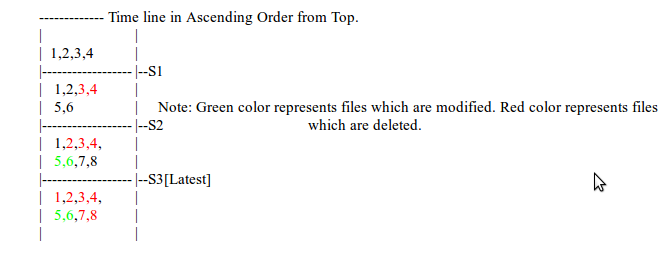
\includegraphics[scale=0.8]{figs/preliminar/Approach2.png}
  \caption{Deletion of Snapshot}
  \label{fig:approach2}
\end{figure}


\subsubsection{\textbf{Deleting an file/Inode}}
If the file is with isDeleted=1 and there is no entry for it in above table then it can be deleted permanently. After deleting file, we will check in D-List, to see if there are any logs with this Inode, if there then we will delete them.The same applies for directory. When user issues a command to delete a directory then mark isDeleted=1 for all of its children.Each children is an Inode, so we If the Inode is with isDeleted=1 and there is no entry for it in above table then it can be deleted permanently. After deleting Inode, we will check in D-List, to see if there are any logs with this Inode, if there then we will delete them

\subsubsection{\textbf{Handling the replication factor change of a file}}

Since we keep latest information about an Inode in Inodes’ table, we need to a mechanism to handle the case of replication factor changes. For example, in S1 the replication factor is 3 , then changed to 6 and S2 was taken , then changed to 9 , then S3 was taken, then changed to 2.
We find value 2 in Inodes’ table. The replication factor= Max(Current value, Max(values in M-List for this Inode)). In this case we will find it as 9 and we expect block report mentioning replication factor of 9 for each block.Suppose S3 was deleted , then the row with value 9 is deleted and we find maximum value 6. 

\subsubsection{\textbf{Disadvantages:}}
1. Time for taking snapshot is O(n) where n is the number of descendants  in directory 


  %%%%%%%%%%%%%%%%%%%%%%%%%%%%%%%%%%%%%%%%%%%%%%%%%%%%%%%%%%%%%%%%%%%%%%%%%%%%%
  %
%%%%%                      SECOND SECTION
 %%%
  %



  %%%%%%%%%%%%%%%%%%%%%%%%%%%%%%%%%%%%%%%%%%%%%%%%%%%%%%%%%%%%%%%%%%%%%%%%%%%%%
  %
%%%%%                         ANOTHER SECTION
 %%%
  %


  %%%%%%%%%%%%%%%%%%%%%%%%%%%%%%%%%%%%%%%%%%%%%%%%%%%%%%%%%%%%%%%%%%%%%%%%%%%%%
  %
%%%%%                          LAST SECTION
 %%%
  %


  %
 %%%
%%%%%                        THE END
  %
  %%%%%%%%%%%%%%%%%%%%%%%%%%%%%%%%%%%%%%%%%%%%%%%%%%%%%%%%%%%%%%%%%%%%%%%%%%%%%

%%% Local Variables: 
%%% mode: latex
%%% TeX-master: "tese"
%%% End: 
